\documentclass[]{article}
\usepackage{graphicx}

%opening
\title{MTH 343 Numerical Analysis Chapter 1: Mathematical Preliminaries \& Error Analysis}
\author{Sheikh Abdul Raheem Ali}

\begin{document}

\maketitle

\begin{abstract}
	Numerical Analysis is a way to do math problems on a computer. 
\end{abstract}


Two types of solutions: Analytical (Exact) and Approximate (Numerical).


\[ Example: \int_{0}^{1} \! 2x(1+x)^{-1/2} \ dx \]

We may solve this \textbf{Analytically} using u-substitution: 

\[ u = 1 + x^2, \ du = 2x \]

\[\int \! 2x(1+x)^{-1/2} \ dx = \int \! u^{-1/2} du  = \frac{u^{1/2}}{\frac{1}{2}} \]

\[ = \left. 2\sqrt{1+x^2} \right|_{0}^1 = 2\sqrt{2} - 2 \]

\begin{figure}
	\centering
	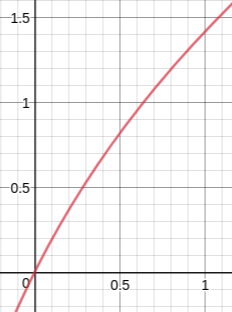
\includegraphics[width=\linewidth]{graph.png}
	\caption{Graph of $ 2x(1+x)^{-1/2} $ from 0 to 1. The numerical solution would be to graph the function and estimate the area using slices, AKA a Riemann sum.  }
	\label{fig:graph}
\end{figure}

\section*{Numerical Solution:}

\subsection*{Advantages:}

\begin{enumerate}
	\item Results approach arbitrary precision with the help of a computer.
	\item An answer can be obtained even when a problem has no exact solution.
\end{enumerate}

\subsection*{Disadvantages:}


\begin{enumerate}
	\item It is \underline{only} an approximate solution.
	\item The solution's behavior is not known.  
\end{enumerate}


\section*{Analytical Solution:}

\subsection*{Advantages:}

\begin{enumerate}
	\item It is exact.
	\item The solution's properties (e.g behavior at infinity, where it is continuous, maxima-minima) are known. 
\end{enumerate}

\subsection*{Disadvantages:}


\begin{enumerate}
	\item Is difficult to determine.
	\item Often does not exist (Example $ \displaystyle{\int_{0}^{\pi} \! \sqrt{1 + \cos^2(x)} dx} $ or $ \displaystyle{\int \! e^{x^3} dx}$) so numerical is the best we can do.
	\item Even if a closed form solution is known, most of the time you have to approximate it in order to interpret it. 
\end{enumerate}

One integral that we got after 140 years: $ \int \! e^{-x^2} \ dx$ (using polar-co-ordinates). 



\end{document}
